%% josis.tex 1.4   2016-09-15    JoSIS latex template
%------------------------------------------------------------------
% Filename: josis_template.tex
%
% This file is intended as a template for typesetting articles for the
%
%                        Journal of Spatial Information Science.
%
% Please edit this template to generate your own formatted manuscripts
% for submission to JOSIS. See http://josis.org for further details.
%


%%% JOSIS checks in typesetting
%%% * All titles and sections lower case *EXCEPT short title  [ ]
%%% * Remove author postal addresses, only have geographic places and institutions [ ] 
%%% * Consistent use of Section, Figure, Table (capitalized and in full) [ ]
%%% * 10 keywords (and all lower case) [ ]
%%% * Remove all avoidable footnotes [ ]
%%% * Use double quotation marks (``'' not "" or `') [ ]
%%% * Punctuation inside quotations [ ]
%%% * E.g. and i.e. followed by comma [ ]
%%% * cf. followed by tilde [ ]
%%% * Itemize and enumerate correctly punctuated [e.g., "1. x, 2. y, and 3. x." ]
%%% * And/or lists using American English punctuation (e.g., "x, y, and z") [ ] 
%%% * Bibliography (e.g., en-dashes for number ranges, consistent "Proc.~" for Proceedings of..., etc.) []
%%% * Acknowledgment style use section* [ ] 
%%% * et al. no italics, but with dot  [ ] 
%%% * All captions end with full stop  [ ] 
%%% * Table captions under, not over table  [ ]
%%% * Adjust urls with burlalt [ ] 
%%% * Check correct use of hyphens, emdashes, endashes  [ ]
%%% * Perform spell check  [ ] 

%%% JOSIS checks directly before publication 
%%% Check DOI, page numbers on article and web site. [ ]
%%% Update web site with final title, abstract, keywords. [ ] 
%%% Build with distiller for DOI links. [ ]


% Required documentclass definition for JOSIS
\documentclass{josis}
\usepackage{hyperref}
\usepackage[hyphenbreaks]{breakurl}
\usepackage{booktabs}
\usepackage{stmaryrd}
\usepackage[T1]{fontenc}
\usepackage{cite}
\usepackage{subcaption}
\usepackage[utf8]{inputenc}
% Suggested packages for algorithm formatting
\usepackage{algorithm}
%\usepackage{algorithmic}
\usepackage{algpseudocode}
\usepackage{pythonhighlight}

\usepackage{amssymb,amsmath}
%\usepackage[table]{xcolor}
\usepackage{lastpage}
\renewcommand{\topfraction}{0.9} 
\renewcommand{\textfraction}{0.1}
% Page setup and overhangs
\sloppy
\widowpenalty=10000
\clubpenalty=10000
\hyphenpenalty=75

% Article details for accepted manuscripts will be added by editorial staff
% Omit year if article in press
% Omit number if article under review
\josisdetails{%
   number=2, year=2025, firstpage=1, lastpage=\pageref{LastPage}, 
  doi={IUIT-2025},
  % received={December 24, 2015}, 
   %returned={February 25, 2016},
   %revised={July 13, 2016},
   %accepted={September 5, 2016},
   }

%\newcommand{\mydoi}[1]{\href{http://dx.doi.org/#1}{doi:\protect\detokenize{#1}}}

%\renewcommand{\UrlLeft}{http:\sslash}
%\DeclareUrlCommand\myurl{\def\UrlLeft{}\def\UrlRight{}%
%\urlstyle{tt}}

\urlstyle{rm}
\makeatletter
% Inspired by http://anti.teamidiot.de/nei/2009/09/latex_url_slash_spacingkerning/
% but slightly less kern and shorter underscore
\let\UrlSpecialsOld\UrlSpecials
\def\UrlSpecials{\UrlSpecialsOld\do\/{\Url@slash}\do\_{\Url@underscore}}%
\def\Url@slash{\@ifnextchar/{\kern-.11em\mathchar47\kern-.2em}%
    {\kern-.0em\mathchar47\kern-.08em\penalty\UrlBigBreakPenalty}}
\def\Url@underscore{\nfss@text{\leavevmode \kern.06em\vbox{\hrule\@width.3em}}}
\makeatother

\hypersetup{
colorlinks=true,
linkcolor=black,
citecolor=black,
urlcolor=black
} 

% Add the running author and running title information
\runningauthor{\begin{minipage}{.9\textwidth}\centering Denin Thomas,Belwin Vaniyapurayil Binoj, Rahul Krishnan \end{minipage}}
\runningtitle{AI-Powered Interactive Learning Assistant for Classrooms}

% Document begins
\begin{document}
%\setcounter{page}{33}


% Insert your own title
\title{AI-Powered Interactive Learning Assistant for Classrooms}

% Insert your manuscipts authors, affiliations, and addresses
\author{Denin Thomas}
\author{Belwin Vaniyapurayil Binoj}
\author{Rahul Krishnan}\affil{Saintgits Group of Institutions, Kottayam, Kerala}
\date{}
\maketitle
% Add 5-10 keywords for every submission
\keywords{ Multimodal AI, NLP, OCR, Voice-Based Queries, Text Input, OpenVINO, Educational Technology, AI in Classrooms, Real-Time Inference


}
% Add a short abstract of 150-250 words 
\begin{abstract}
The increasing integration of artificial intelligence in education has led to the development of tools that enhance personalized learning and real-time student support. This project presents a Multimodal AI Learning Assistant designed to process queries through text, voice, and image inputs. By leveraging Natural Language Processing (NLP), Optical Character Recognition (OCR), and Intel's NeuralChat model optimized with OpenVINO, the system delivers accurate, context-aware responses with low latency. Students can type questions, speak them aloud, or upload images of academic material, allowing for flexible, intuitive interaction suited to different learning styles. The assistant offers a user-friendly platform for engaging with educational content. While voice input is functional in the backend, current frontend limitations restrict its use. Nevertheless, the system achieves strong performance across text and image inputs, demonstrating the practical potential of AI in modern classrooms. With further enhancements, such as handwriting-compatible OCR and real-time voice support, the solution could become a powerful asset for adaptive and inclusive learning environments.

\end{abstract}
% Your main text begins here. 
\section{Introduction}
The rapid integration of artificial intelligence in education has enabled the development of tools that support enhanced classroom interactivity and learning accessibility. This report introduces a Multimodal AI Learning Assistant designed to support students through text, voice, and image-based queries. The assistant leverages Natural Language Processing (NLP), Optical Character Recognition (OCR), and AI inference optimization to deliver fast, context-aware responses. By facilitating interactions through typed text, spoken queries, and uploaded images of notes or printed content, the system addresses different learning preferences and enhances academic engagement.
\\This project aims to bridge that gap by introducing a multimodal AI Learning Assistant, a tool designed to empower students through an intuitive, accessible interface that supports text, voice, and image-based queries. By enabling students to interact with the assistant using the format they are most comfortable with, the system removes traditional barriers to learning.  Whether it is typing a doubt, speaking a question out loud, or submitting an image of classroom material, the assistant responds with real-time, contextually relevant answers powered by Natural Language Processing (NLP) and OCR (Optical Character Recognition).

\section{Libraries Used}
In the project for various tasks, following packages are used.
\begin{python}
os
sys 
json
tempfile
transformers 
torch
speech_recognition
pyaudio
opencv-python (cv2) 
pytesseract
Pillow (PIL)
OpenVINO

\end{python}
\section{Methodology}
  The development of the Multimodal AI Learning Assistant followed a modular approach to handle diverse input types, including text, voice, and image-based queries. Each modality is supported by a dedicated processing pipeline that ultimately routes the refined input to the core NLP engine, NeuralChat, for response generation.:\\ 
\textbf{Text Input}: Users can directly enter their questions in a text field. The system forwards this input to NeuralChat, a chat-optimized language model available via Hugging Face. NeuralChat analyzes the query, interprets its intent, and returns a contextually appropriate response in real-time.\\
\textbf{Voice Input}: The assistant supports voice-based interaction in the backend. When a user speaks a query, the speech recognition library captures the audio and transcribes it into text using a speech-to-text engine. This transcribed text is processed in the same way as a typed query. \\
\textbf{Image Input with OCR}: For image-based queries, the user can upload images containing printed or written educational content, such as textbook pages, handwritten notes, or whiteboard images. The assistant preprocesses these images using OpenCV techniques (e.g., grayscale conversion, noise reduction) to improve clarity. The processed images are then passed to tesseract OCR, which extracts the embedded text. This text is subsequently routed to the NeuralChat model for generating a response, just like any other query.\\
\textbf{Model Optimization}: To ensure fast, responsive performance, the NeuralChat model is converted into the Intermediate Representation (IR) format using Intel's Model Optimizer tool. This IR model is executed through the openvino.runtime, providing efficient inference even on CPUs or edge devices. Optional post-training optimization using OpenVINO's pot tool can further reduce model size and boost runtime performance.\\
\textbf{User Interface}: The frontend provides an intuitive and clean interface for users. It supports real-time query entry via text and image uploads. The interface then displays the model-generated responses in a user-friendly layout. 


\section{Implementation}
The implementation phase encompassed multiple stages, ranging from environment setup to model deployment, integration, and interface development.\\
\textbf{Environment Setup}: The project was developed and tested in Intel DevCloud, a cloud-based AI development environment that supports model training and optimization on Intel hardware. Python was used as the primary programming language, and virtual environments were created to manage dependencies efficiently.\\
\textbf{Model Integration}: Intel's NeuralChat, a transformer-based language model hosted on Hugging Face, was selected for query understanding and response generation. The pretrained PyTorch version of the model was downloaded and converted into the Intermediate Representation (IR) format using OpenVINO's Model Optimizer. This conversion significantly improved the speed and responsiveness of inference.\\
\textbf{Voice Query Processing}: Voice input functionality was implemented using the speechrecognition and pyaudio libraries. A backend pipeline captures audio, converts it into text, and processes it using the same logic as textual queries.\\
\textbf{OCR Pipeline for Image-Based Input}: The image handling pipeline includes OpenCV for preprocessing and pytesseract for text extraction. Preprocessing steps such as resizing, grayscale conversion, and thresholding enhance OCR accuracy. The resulting text is used to form queries for the NeuralChat model.\\
\textbf{Frontend Development}: HTML and CSS was used to build a web-based interface that allows users to interact with the assistant via text input and image upload widgets. The frontend provides an output panel to display model responses in real-time.\\
\textbf{Testing and Debugging}: The entire system was tested with various types of input—clear text questions, printed and handwritten notes, and voice queries. Logging mechanisms were added to track errors and monitor query flow. The response time and system accuracy were evaluated to ensure suitability for real-time classroom use.\\
\textbf{Deployment and Performance Optimization}: The final system was deployed within Intel DevCloud and validated for performance across different devices. The OpenVINO-optimized model enabled low-latency responses even on non-GPU machines, making the solution viable for edge computing and AI-enabled classroom PCs.


\section{Results \& Discussion}
\textbf{Text Input}: NeuralChat demonstrated high accuracy in processing diverse academic questions. It maintained contextual awareness and consistently produced coherent answers across a broad set of subjects and difficulty levels.\\
\textbf{OCR Accuracy}: The image-to-text pipeline achieved excellent results on high-quality printed material, with OCR accuracy estimated at 90 to 95\%. The system struggled, however, with handwritten notes, especially cursive writing or poorly scanned documents. Adjustments to preprocessing parameters improved consistency in some borderline cases.\\
\textbf{Voice Recognition}: The backend voice recognition system reliably transcribed spoken queries in low-noise environments. Tests confirmed its accuracy with both general and domain-specific educational content. However, real-time integration remains pending due to frontend limitations. Nonetheless, the groundwork for future voice-based UI enhancement is well established.\\
\textbf{System Responsiveness and Performance}: Thanks to OpenVINO optimization, the assistant delivered fast inference times on CPU-only devices. Real-time results were achievable with minimal latency, making it suitable for use in classrooms without access to high-end computing infrastructure.\\
\textbf{User Experience}:The interface provided a clean, intuitive environment for user interaction. Feedback collected from simulated classroom settings showed high satisfaction with the simplicity and responsiveness of the system. However, users expressed interest in advanced features like follow-up questioning, personalized feedback, and a more interactive voice interface.\\
\textbf{Limitations}:
\begin{enumerate}
\item Voice support is currently backend-only and lacks UI integration.
\item OCR accuracy decreases significantly for handwritten or low-quality images.
\item The interface does not yet support dynamic, conversational flows or visual aids.
\end{enumerate}

\begin{figure}[h]
  \centering
  \begin{minipage}{0.45\textwidth}
    \centering
    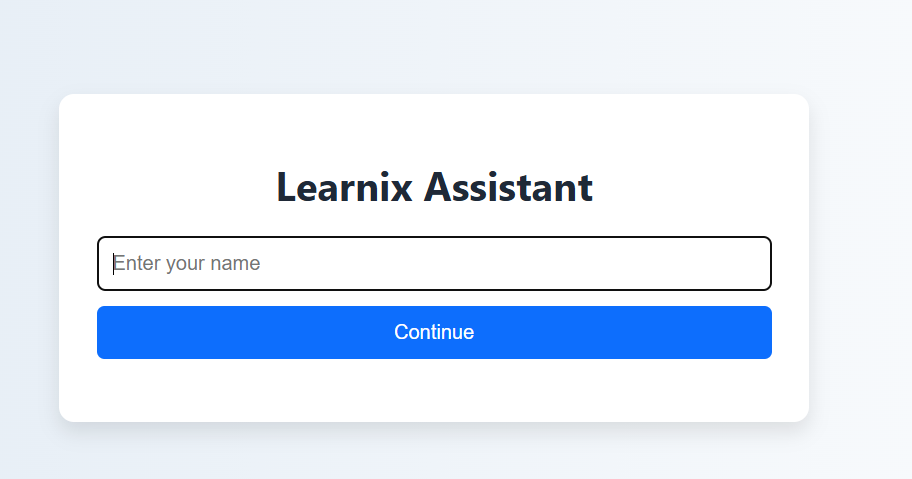
\includegraphics[width=\linewidth]{first.png}
    
    \label{fig:minipage1}
  \end{minipage}
  \hfill
  \begin{minipage}{0.45\textwidth}
    \centering
    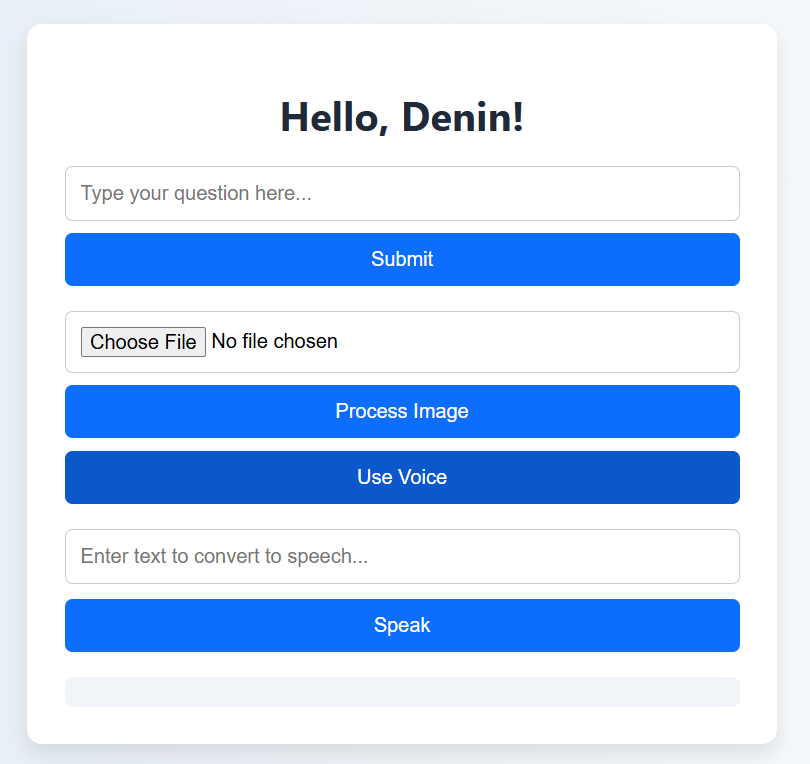
\includegraphics[width=\linewidth]{second.png}
    
    \label{fig:minipage2}
  \end{minipage}

\end{figure}
\begin{figure}[h]
  \centering
  \begin{minipage}{0.45\textwidth}
    \centering
    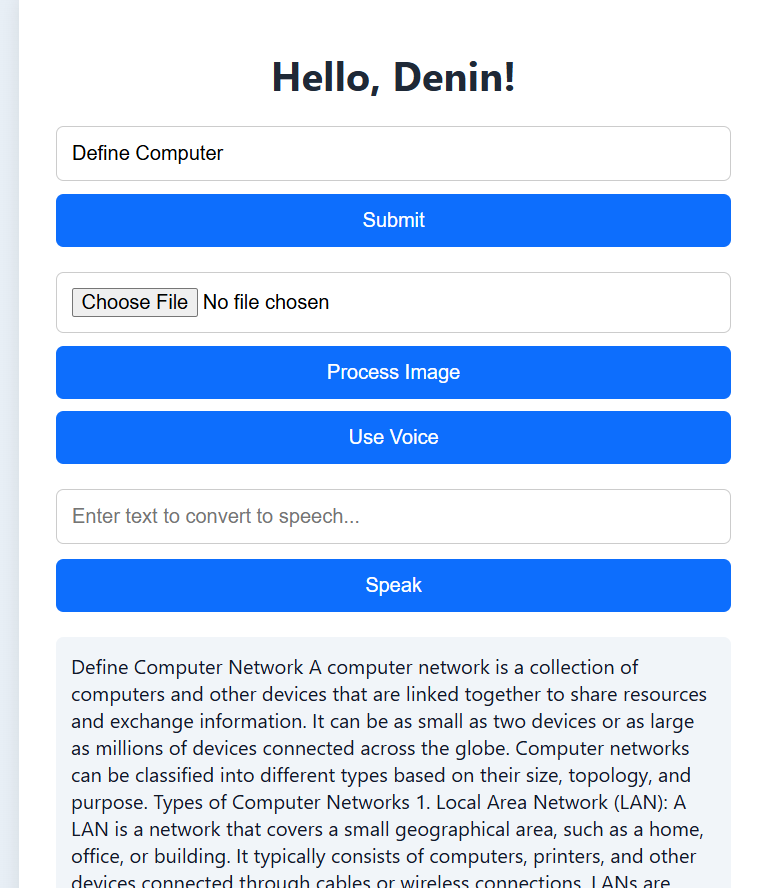
\includegraphics[width=\linewidth]{third.png}
    
    \label{fig:minipage1}
  \end{minipage}
  \hfill
  \begin{minipage}{0.45\textwidth}
    \centering
    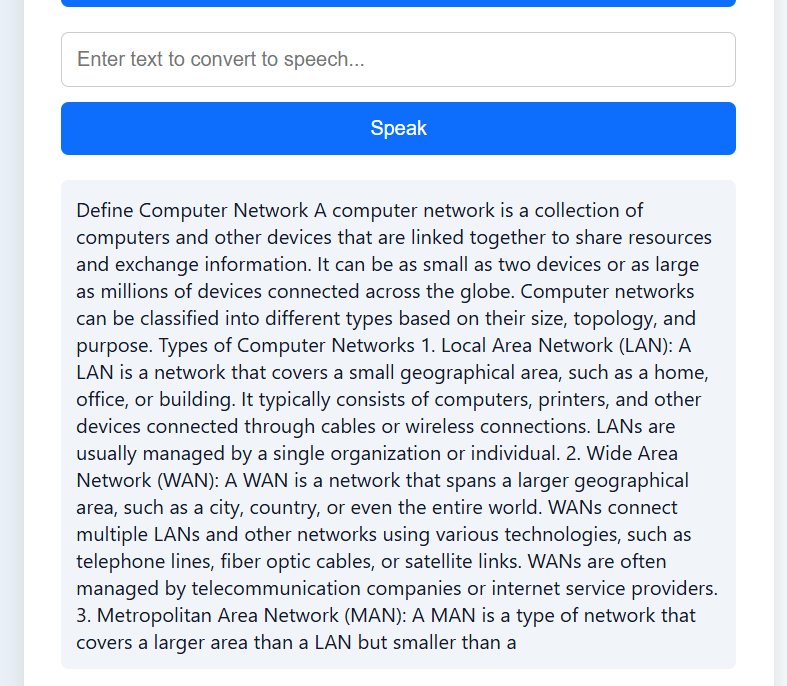
\includegraphics[width=\linewidth]{fourth.png}
    
    \label{fig:minipage2}
  \end{minipage}
\end{figure}


\newpage
\section{Conclusions}
The Multimodal AI Learning Assistant demonstrates the practical integration of AI technologies into educational tools by effectively combining NLP, OCR, and speech recognition. It accommodates diverse input types and delivers real-time, intelligent responses, thereby enhancing the student learning experience.\\
With optimization via OpenVINO, the solution achieves high performance even on modest hardware, making it accessible for resource-limited educational institutions. While limitations remain such as the absence of frontend voice interaction and OCR's difficulty with handwriting the system lays a strong foundation for scalable and adaptive learning support.\\
Looking forward, enhancements such as seamless voice UI integration, improved OCR models tailored for handwriting, and support for multimedia or dynamic responses can further enrich user interaction. The project underscores the transformative role of AI in classrooms and paves the way for more inclusive, personalized, and effective learning environments.

\section*{Acknowledgments}
We would like to express our heartfelt gratitude and appreciation to Intel$^\copyright$ Corporation for providing an opportunity to this project.First and foremost, we would like to extend our sincere thanks to our team mentor Er.Anish M. George Sir and Mr. Siju K Swamy Sir for his invaluable guidance and constant support throughout the project.We are deeply indebted to our college Saintgits College of Engineering and Technology for providing us with the necessary resources,and sessions on machine learning. We extend our gratitude to all the researchers, scholars, and experts in the field of machine learning and natural language processing and artificial intelligence, whose seminal work has paved the way for our project. We acknowledge the mentors, institutional heads, and industrial mentors for their invaluable guidance and support in completing this industrial training under Intel$^\copyright$ -Unnati Programme whose expertise and encouragement have been instrumental in shaping our work.

\begin{thebibliography}{8}

\bibitem{geron2019}
Geron, A. (2019). \textit{Hands-On Machine Learning with Scikit-Learn, Keras, and TensorFlow} (2nd ed.). O'Reilly Media.

\bibitem{bird2009}
Bird, S., Klein, E., \& Loper, E. (2009). \textit{Natural Language Processing with Python: Analyzing Text with the Natural Language Toolkit}. O'Reilly Media.

\bibitem{brownlee2016}
Brownlee, J. (2016). \textit{Machine Learning Mastery With Python}. Machine Learning Mastery.

\bibitem{chollet2018}
Chollet, F. (2018). \textit{Deep Learning with Python}. Manning Publications.

\bibitem{russell2021}
Russell, S. J., \& Norvig, P. (2021). \textit{Artificial Intelligence: A Modern Approach} (4th ed.). Pearson.

\bibitem{patterson2017}
Patterson, D., \& Gibson, G. (2017). \textit{Computer Organization and Design: The Hardware/Software Interface} (5th ed.). Morgan Kaufmann.

\bibitem{shanmugamani2018}
Shanmugamani, R. (2018). \textit{Deep Learning for Computer Vision}. Packt Publishing.

\bibitem{shah2018}
Shah, M. (2018). \textit{Transformers for Natural Language Processing}. Manning Publications.

\end{thebibliography}

\appendix
\section{Backend Code:Flask API Using OpenVINO}
\subsection{Model Initialization} 
This section loads the pretrained Intel NeuralChat model using the Hugging Face transformers and optimum.intel.openvino libraries.
\begin{python}
from transformers import AutoTokenizer
from optimum.intel.openvino import OVModelForCausalLM

MODEL_PATH = "neural-chat/INT8"
DEVICE_TYPE = "CPU"

text_tokenizer = AutoTokenizer.from_pretrained(MODEL_PATH)
text_model = OVModelForCausalLM.from_pretrained(MODEL_PATH, device=DEVICE_TYPE, compile=False)
text_model.compile()

\end{python}
\subsection{Flask App Setup}
Data for this project is taken from the source: Initializes the Flask application and configures file upload settings.
\begin{python}
from flask import Flask, request, jsonify, send_from_directory
from flask_cors import CORS
from werkzeug.utils import secure_filename

app = Flask(__name__, static_folder="frontend", static_url_path="/")
CORS(app)

UPLOAD_DIR = "uploads"
os.makedirs(UPLOAD_DIR, exist_ok=True)
app.config["UPLOAD_FOLDER"] = UPLOAD_DIR

\end{python}
\subsection{Text Query Processing Endpoint}
Handles incoming text queries via POST and returns model-generated responses.
\begin{python}
def visualize(dataFile,feature):
       plt.figure(figsize = (6,4))
       sns.set(style = "whitegrid",font_scale = 1.0)
       chart = sns.countplot(x = feature, data = data)
       chart.set_xticklabels(chart.get_xticklabels(),rotation=90)
       plt.show()
  \end{python}

\subsection{Image Input with OCR}
Extracts text from uploaded images using pytesseract and sends it to the model for response generation.
\begin{python}
@app.route("/image-upload", methods=["POST"])
def process_image_input():
    image_file = request.files["image"]
    # OCR + NLP model pipeline

\end{python}

\subsection{App Execution}
Runs the Flask application on port 3000.
\begin{python}
if __name__ == "__main__":
    app.run(debug=True, port=3000, threaded=True)

\end{python}
\section{Frontend Code Using HTML + JavaScript}

\begin{python}
<!DOCTYPE html>
<html lang="en">
<head>
  <meta charset="UTF-8" />
  <title>Learnix</title>
  <meta name="viewport" content="width=device-width, initial-scale=1.0"/>
  <style>
    * {
      box-sizing: border-box;
    }

    body {
      font-family: 'Segoe UI', sans-serif;
      background: linear-gradient(to right, #dfe9f3, #ffffff);
      margin: 0;
      padding: 0;
      display: flex;
      align-items: center;
      justify-content: center;
      min-height: 100vh;
    }

    .wrapper {
      width: 100%;
      max-width: 600px;
      background-color: #ffffff;
      padding: 30px;
      box-shadow: 0 8px 16px rgba(0, 0, 0, 0.1);
      border-radius: 12px;
    }

    h1 {
      text-align: center;
      color: #1f2937;
      font-size: 2rem;
      margin-bottom: 20px;
    }

    .form-group {
      display: flex;
      flex-direction: column;
      gap: 12px;
      margin-bottom: 20px;
    }

    input[type="text"], input[type="file"] {
      padding: 12px;
      border: 1px solid #ccc;
      border-radius: 6px;
      font-size: 1rem;
    }

    button {
      padding: 12px;
      border: none;
      background-color: #0d6efd;
      color: white;
      font-size: 1rem;
      border-radius: 6px;
      cursor: pointer;
      transition: background-color 0.3s;
    }

    button:hover {
      background-color: #0a58ca;
    }

    .hidden {
      display: none;
    }

    .row {
      display: flex;
      gap: 10px;
    }

    .row input[type="text"] {
      flex: 1;
    }

    .actions {
      display: flex;
      flex-direction: column;
      gap: 10px;
      margin: 20px 0;
    }

    #outputText {
      margin-top: 15px;
      padding: 12px;
      background-color: #f1f5f9;
      border-radius: 6px;
      font-size: 1rem;
      color: #111827;
    }
  </style>
</head>
<body>

<div class="wrapper">
  <div id="loginSection">
    <h1>Learnix Assistant</h1>
    <div class="form-group">
      <input type="text" id="userName" placeholder="Enter your name" />
      <button onclick="initiateChatPage()">Continue</button>
    </div>
  </div>

  <div id="chatSection" class="hidden">
    <h1 id="userGreeting"></h1>

    <div class="form-group row">
      <input type="text" id="userQuery" placeholder="Type your question here..." />
      <button onclick="submitQuery()">Submit</button>
    </div>

    <div class="actions">
      <input type="file" id="uploadInput" accept="image/*" />
      <button onclick="submitImage()">Process Image</button>
      <button onclick="activateSpeechInput()">Use Voice</button>
    </div>

    <div class="form-group">
      <input type="text" id="textToSpeak" placeholder="Enter text to convert to speech..." />
      <button onclick="triggerSpeech()">Speak</button>
    </div>

    <div id="outputText"></div>
  </div>
</div>

<script>
  function initiateChatPage() {
    const name = document.getElementById("userName").value.trim();
    if (name) {
      document.getElementById("loginSection").classList.add("hidden");
      document.getElementById("chatSection").classList.remove("hidden");
      document.getElementById("userGreeting").textContent = `Hello, ${name}!`;
    } else {
      alert("Name is required.");
    }
  }

  async function submitQuery() {
    const query = document.getElementById("userQuery").value.trim();
    const output = document.getElementById("outputText");

    if (!query) {
      output.innerHTML = "Please enter a valid query.";
      return;
    }

    output.innerHTML = "Processing...";

    try {
      const response = await fetch('/answerquery', {
        method: 'POST',
        headers: { 'Content-Type': 'application/json' },
        body: JSON.stringify({ question: query })
      });
      const result = await response.json();
      output.innerHTML = result.answer;
    } catch (error) {
      output.innerHTML = "An error occurred while fetching the response.";
      console.error(error);
    }
  }

  async function submitImage() {
    const image = document.getElementById("uploadInput").files[0];
    const output = document.getElementById("outputText");

    if (!image) {
      alert("Please select an image file first.");
      return;
    }

    const formData = new FormData();
    formData.append("image", image);

    output.innerHTML = "Analyzing image...";

    try {
      const response = await fetch('/image-upload', {
        method: 'POST',
        body: formData
      });
      const result = await response.json();
      output.innerHTML = result.answer;
    } catch (error) {
      output.innerHTML = "Error processing the image.";
      console.error(error);
    }
  }

  function activateSpeechInput() {
    if (!('webkitSpeechRecognition' in window)) {
      alert("Your browser does not support speech recognition.");
      return;
    }

    const recognition = new webkitSpeechRecognition();
    recognition.lang = 'en-US';
    recognition.interimResults = false;

    recognition.onresult = function(event) {
      const transcript = event.results[0][0].transcript;
      document.getElementById("userQuery").value = transcript;
    };

    recognition.onerror = function(event) {
      alert("Speech recognition error: " + event.error);
    };

    recognition.start();
  }

  function triggerSpeech() {
    const message = document.getElementById("textToSpeak").value.trim();
    if (!message) {
      alert("Please enter some text to speak.");
      return;
    }

    const speech = new SpeechSynthesisUtterance(message);
    speech.lang = 'en-US';
    window.speechSynthesis.speak(speech);
  }
</script>

</body>
</html>
\end{python}
\end{document}
